%!TEX root = ../main.tex

\section{Experimental setup}
\label{sec:setup}

\todo{Get setup picture, MOKE pdf p.15}

%\begin{figure}
%	\label{fig:setup}
%	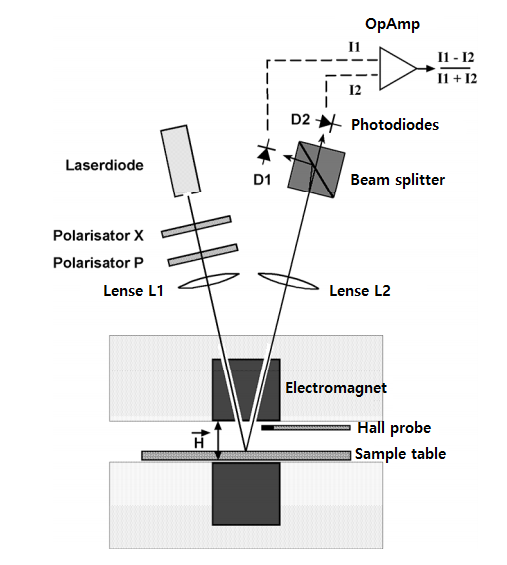
\includegraphics[width=1.0\textwidth]{./img/setup.png}
%	\caption{}{Experimental setup of the MOKE lab}
%\end{figure}

As can be seen in \autoref{fig:setup}, a sample can be placed inside of an
electromagnet with controllable $B$-field. The measurement apparatus that will test
the magneto-optic Kerr effect consists of a laser diode that shines polarised light 
onto the sample. Two polarisation filters and focusing lenses exist to tweak the 
properties of light beam and improve the overall signal strength. The light that gets
reflected off the magnetic sample travels trough a beam splitter into two photo 
diodes that in turn feed a differential amplifier. A Hall probe monitors the strength
of the $B$-field in which the sample is placed.
